\section{Talsperren}


\subsection{Bogenstaumauer}

\begin{minipage}[c]{0.38\columnwidth}
    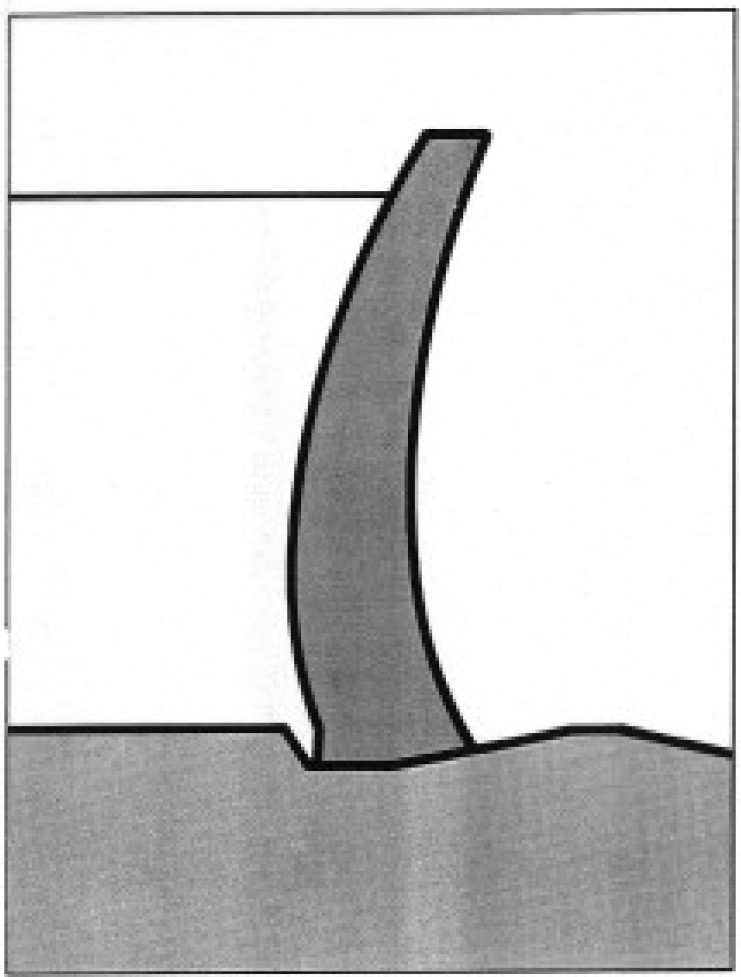
\includegraphics[width=0.98\columnwidth, align=c]{images/Talsperre_1.jpg}
\end{minipage}
\hfill
\begin{minipage}[t]{0.58\columnwidth}
    \begin{itemize}
    \item Beton
    \item Schlank
    \item Kraft wird links und rechts in den Hang geleitet (Gewölbewirkung)
    \item Beispiel: Verzasca Damm (Tessin)
    \end{itemize}
\end{minipage}



\subsection{Gewichtsstaumauer}
\begin{minipage}[c]{0.38\columnwidth}
    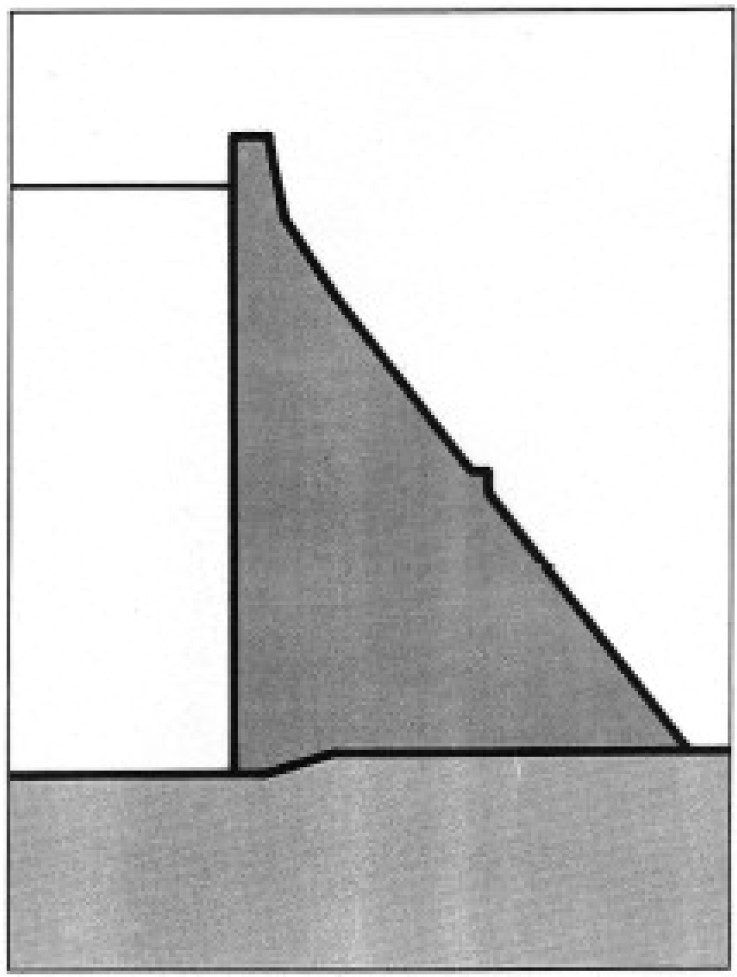
\includegraphics[width=0.98\columnwidth, align=c]{images/Talsperre_2.jpg}
\end{minipage}
\hfill
\begin{minipage}[c]{0.58\columnwidth}
    \begin{itemize}
  \item Beton oder Mauerwerk
  \item Hohes Eigengewicht
  \item Kraft wird durch Eigengewicht gehalten
  \item Beispiel: Grande Dixence (Wallis) Höchste Gewichtsstaumauer der Welt
\end{itemize}

\end{minipage}

\subsection{Staudamm}


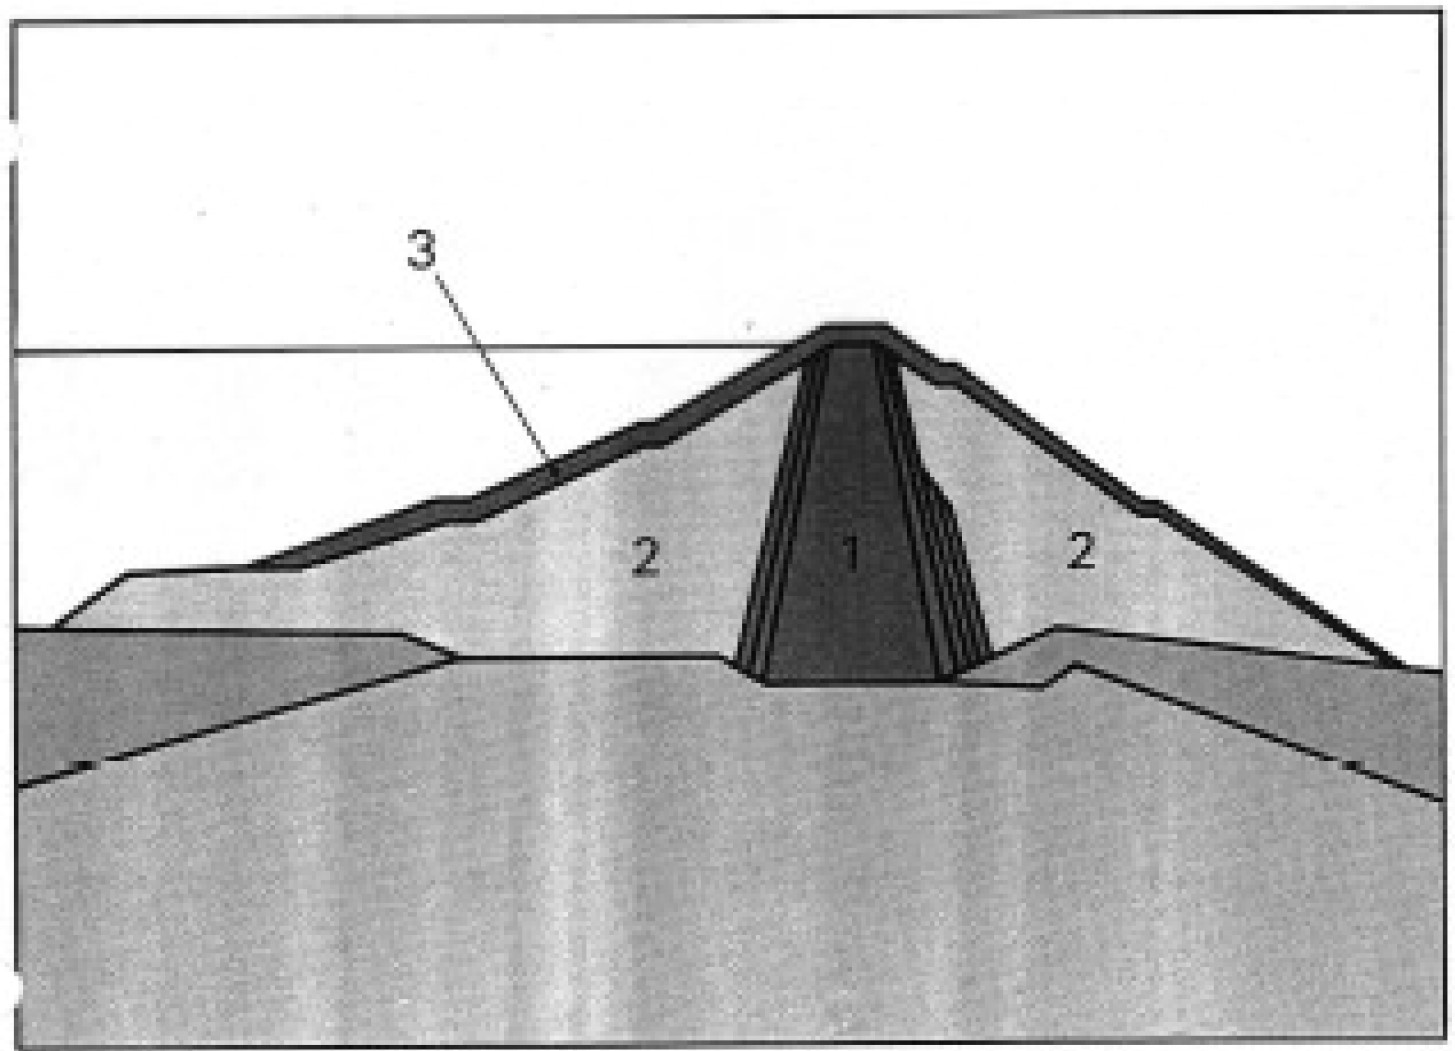
\includegraphics[width=0.8\columnwidth, align=c]{images/Talsperre_3.jpg}

\vspace{0.15cm}

\begin{enumerate}
    \item Kern 
    \item Stützkörper
    \item Schutzschicht
\end{enumerate}

\vspace{0.15cm}

\begin{itemize}
  \item Aufgeschüttet
  \item Flacher Böschungswinkel
  \item Steinschüttung unterschiedlicher Korngrösse
  \item Beispiel: Stausee Mattmark (Wallis) (Höchster Erdschüttdamm der Welt)
\end{itemize}

\vspace{0.15cm}


\subsection{Hochwassersicherheit}

\begin{enumerate}
  \item Überlaufbauwerk, Hochwasserentlastung \\
  => verhindert den Abfluss über Krone
  \item evtl. Mittelablass
  \item Grundablass
\end{enumerate}




\subsection{Wasserfassung}
Wird hier nicht erläutert.

